\documentclass[tikz, border=6pt]{standalone}
\IfFileExists{lmodern.sty}{\usepackage[T1]{fontenc}\usepackage{lmodern}}{}
\usepackage{amsmath,amssymb,bm}
\usepackage[scaled=0.95]{helvet}
\usetikzlibrary{arrows.meta, fit}
\definecolor{Blue}{HTML}{3A76D8}
\definecolor{Orange}{HTML}{EE8133}
\definecolor{Red}{HTML}{DF4B4B}
\definecolor{Gray}{HTML}{6B7280}
\definecolor{Ink}{HTML}{1F2937}
\begin{document}
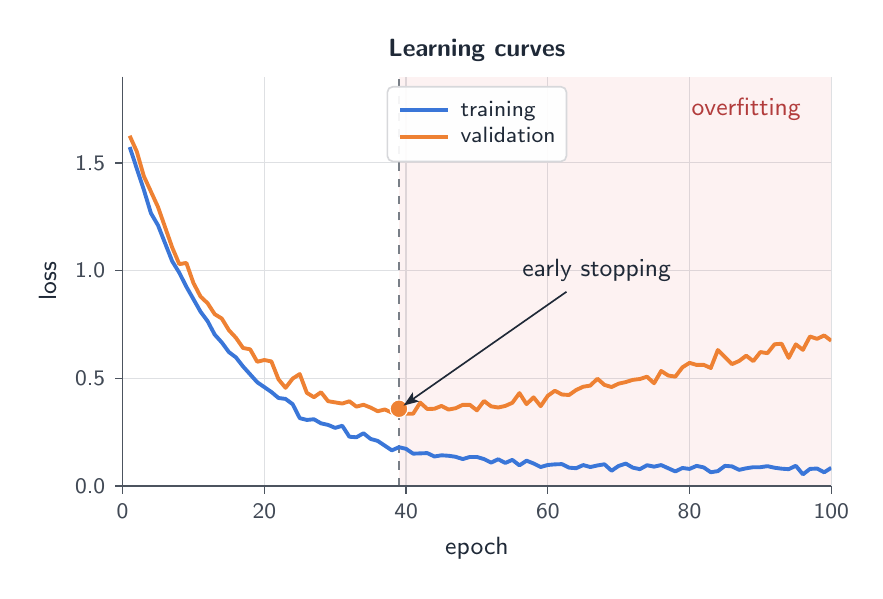
\begin{tikzpicture}[color=Ink, execute at begin picture={\sffamily}, line width=0.6pt, >={Stealth[length=5.5pt, width=4pt, inset=1.2pt]}, line join=round]
  % axes ax1
  \draw[Gray!22, line width=0.4pt] (0,0) -- (0,5.2) (1.8,0) -- (1.8,5.2) (3.6,0) -- (3.6,5.2) (5.4,0)
      -- (5.4,5.2) (7.2,0) -- (7.2,5.2) (9,0) -- (9,5.2) (0,0) -- (9,0) (0,1.368) -- (9,1.368)
      (0,2.737) -- (9,2.737) (0,4.105) -- (9,4.105);
  \begin{scope}
    \clip (0,0) rectangle (9,5.2);
    \fill[fill=Red, fill opacity=0.07] (3.51,0) -- (9,0) -- (9,5.2) -- (3.51,5.2) -- cycle;
    \draw[dashed, color=Ink!60, line width=0.9pt] (3.51,0) -- (3.51,5.2);
    \draw[color=Blue, line width=1.4pt] (0.09,4.307) -- (0.27,3.764) -- (0.36,3.467) -- (0.45,3.313) --
        (0.63,2.857) -- (0.72,2.711) -- (0.81,2.533) -- (0.99,2.216) -- (1.08,2.095) -- (1.17,1.925) --
        (1.26,1.825) -- (1.35,1.703) -- (1.44,1.635) -- (1.53,1.52) -- (1.71,1.32) -- (1.89,1.196) --
        (1.98,1.12) -- (2.07,1.108) -- (2.16,1.041) -- (2.25,0.864) -- (2.34,0.841) -- (2.43,0.85) --
        (2.52,0.798) -- (2.61,0.778) -- (2.7,0.74) -- (2.79,0.767) -- (2.88,0.628) -- (2.97,0.621) --
        (3.06,0.672) -- (3.15,0.6) -- (3.24,0.575) -- (3.42,0.455) -- (3.51,0.495) -- (3.6,0.474) --
        (3.69,0.413) -- (3.87,0.42) -- (3.96,0.377) -- (4.05,0.392) -- (4.14,0.386) -- (4.23,0.373) --
        (4.32,0.344) -- (4.41,0.371) -- (4.5,0.371) -- (4.59,0.344) -- (4.68,0.299) -- (4.77,0.342) --
        (4.86,0.295) -- (4.95,0.334) -- (5.04,0.264) -- (5.13,0.324) -- (5.22,0.288) -- (5.31,0.243) --
        (5.4,0.269) -- (5.49,0.277) -- (5.58,0.28) -- (5.67,0.235) -- (5.76,0.228) -- (5.85,0.268) --
        (5.94,0.243) -- (6.03,0.263) -- (6.12,0.278) -- (6.21,0.196) -- (6.3,0.257) -- (6.39,0.287) --
        (6.48,0.235) -- (6.57,0.216) -- (6.66,0.266) -- (6.75,0.248) -- (6.84,0.268) -- (7.02,0.187) --
        (7.11,0.231) -- (7.2,0.219) -- (7.29,0.258) -- (7.38,0.238) -- (7.47,0.177) -- (7.56,0.191) --
        (7.65,0.258) -- (7.74,0.251) -- (7.83,0.207) -- (7.92,0.227) -- (8.01,0.241) -- (8.1,0.241) --
        (8.19,0.254) -- (8.28,0.234) -- (8.37,0.222) -- (8.46,0.216) -- (8.55,0.259) -- (8.64,0.15) --
        (8.73,0.219) -- (8.82,0.224) -- (8.91,0.176) -- (9,0.233);
    \draw[color=Orange, line width=1.4pt] (0.09,4.45) -- (0.18,4.251) -- (0.27,3.937) -- (0.45,3.545) --
        (0.63,3.032) -- (0.72,2.82) -- (0.81,2.835) -- (0.9,2.58) -- (0.99,2.408) -- (1.08,2.323) --
        (1.17,2.184) -- (1.26,2.129) -- (1.35,1.981) -- (1.44,1.884) -- (1.53,1.755) -- (1.62,1.738) --
        (1.71,1.58) -- (1.8,1.602) -- (1.89,1.584) -- (1.98,1.357) -- (2.07,1.249) -- (2.16,1.366) --
        (2.25,1.424) -- (2.34,1.185) -- (2.43,1.13) -- (2.52,1.193) -- (2.61,1.079) -- (2.79,1.049) --
        (2.88,1.078) -- (2.97,1.01) -- (3.06,1.034) -- (3.15,0.998) -- (3.24,0.952) -- (3.33,0.974) --
        (3.42,0.934) -- (3.51,0.983) -- (3.6,0.919) -- (3.69,0.92) -- (3.78,1.061) -- (3.87,0.98) --
        (3.96,0.983) -- (4.05,1.019) -- (4.14,0.973) -- (4.23,0.99) -- (4.32,1.033) -- (4.41,1.033) --
        (4.5,0.963) -- (4.59,1.082) -- (4.68,1.014) -- (4.77,0.999) -- (4.86,1.019) -- (4.95,1.059) --
        (5.04,1.182) -- (5.13,1.042) -- (5.22,1.128) -- (5.31,1.016) -- (5.4,1.148) -- (5.49,1.212) --
        (5.58,1.164) -- (5.67,1.158) -- (5.76,1.221) -- (5.85,1.263) -- (5.94,1.277) -- (6.03,1.365) --
        (6.12,1.286) -- (6.21,1.259) -- (6.3,1.302) -- (6.39,1.322) -- (6.48,1.35) -- (6.57,1.361) --
        (6.66,1.39) -- (6.75,1.307) -- (6.84,1.463) -- (6.93,1.405) -- (7.02,1.391) -- (7.11,1.509) --
        (7.2,1.566) -- (7.29,1.54) -- (7.38,1.541) -- (7.47,1.501) -- (7.56,1.729) -- (7.74,1.55) --
        (7.83,1.59) -- (7.92,1.657) -- (8.01,1.588) -- (8.1,1.703) -- (8.19,1.689) -- (8.28,1.802) --
        (8.37,1.809) -- (8.46,1.629) -- (8.55,1.801) -- (8.64,1.731) -- (8.73,1.901) -- (8.82,1.871) --
        (8.91,1.914) -- (9,1.847);
    \filldraw[fill=Orange, draw=white, line width=0.4pt] (3.51,0.983) circle[radius=3.2pt];
  \end{scope}
  \draw[Ink!80, line width=0.5pt] (0,5.2) -- (0,0) -- (9,0);
  \draw[Ink!80, line width=0.5pt] (0,0) -- (0,-0.1) (1.8,0) -- (1.8,-0.1) (3.6,0) -- (3.6,-0.1)
      (5.4,0) -- (5.4,-0.1) (7.2,0) -- (7.2,-0.1) (9,0) -- (9,-0.1) (0,0) -- (-0.1,0) (0,1.368) --
      (-0.1,1.368) (0,2.737) -- (-0.1,2.737) (0,4.105) -- (-0.1,4.105);
  \node[anchor=north, font=\footnotesize, text=Ink!85, inner sep=2pt] (ax1-xt0) at (0,-0.14) {0};
  \node[anchor=north, font=\footnotesize, text=Ink!85, inner sep=2pt] (ax1-xt1) at (1.8,-0.14) {20};
  \node[anchor=north, font=\footnotesize, text=Ink!85, inner sep=2pt] (ax1-xt2) at (3.6,-0.14) {40};
  \node[anchor=north, font=\footnotesize, text=Ink!85, inner sep=2pt] (ax1-xt3) at (5.4,-0.14) {60};
  \node[anchor=north, font=\footnotesize, text=Ink!85, inner sep=2pt] (ax1-xt4) at (7.2,-0.14) {80};
  \node[anchor=north, font=\footnotesize, text=Ink!85, inner sep=2pt] (ax1-xt5) at (9,-0.14) {100};
  \node[anchor=east, font=\footnotesize, text=Ink!85, inner sep=2pt] (ax1-yt0) at (-0.14,0) {0.0};
  \node[anchor=east, font=\footnotesize, text=Ink!85, inner sep=2pt] (ax1-yt1) at (-0.14,1.368) {0.5};
  \node[anchor=east, font=\footnotesize, text=Ink!85, inner sep=2pt] (ax1-yt2) at (-0.14,2.737) {1.0};
  \node[anchor=east, font=\footnotesize, text=Ink!85, inner sep=2pt] (ax1-yt3) at (-0.14,4.105) {1.5};
  \node[font=\small, anchor=west] (ann1) at (4.95,2.737) {early stopping};
  \draw[->, shorten >=2pt] (ann1) -- (3.51,0.983);
  \node[font=\small, text=Red!80!black] at (7.92,4.789) {overfitting};
  \node[fit=(ax1-xt0)(ax1-xt1)(ax1-xt2)(ax1-xt3)(ax1-xt4)(ax1-xt5), inner sep=0pt] (ax1-xticks) {};
  \node[anchor=north, font=\small, align=center, inner sep=4pt] at (4.5,0 |- ax1-xticks.south) {epoch};
  \node[fit=(ax1-yt0)(ax1-yt1)(ax1-yt2)(ax1-yt3), inner sep=0pt] (ax1-yticks) {};
  \node[anchor=south, rotate=90, font=\small, align=center, inner sep=4pt] at (ax1-yticks.west |- 0,2.6) {loss};
  \node[anchor=south, font=\small\bfseries, inner sep=4pt, align=center] at (4.5,5.25) {Learning curves};
  \node[anchor=north, font=\footnotesize, inner sep=4pt, align=left, fill=white, draw=Ink!18, rounded corners=2pt, fill opacity=0.92, text opacity=1] at (4.5,5.08) {%
    \begin{tabular}{@{}l@{\hspace{4pt}}l@{}}
      \tikz[baseline=-0.6ex]{\draw[color=Blue, line width=1.4pt] (0,0) -- (0.6,0);} & training \\
      \tikz[baseline=-0.6ex]{\draw[color=Orange, line width=1.4pt] (0,0) -- (0.6,0);} & validation \\
    \end{tabular}%
  };
\end{tikzpicture}
\end{document}
